% Options for packages loaded elsewhere
\PassOptionsToPackage{unicode}{hyperref}
\PassOptionsToPackage{hyphens}{url}
\PassOptionsToPackage{dvipsnames,svgnames*,x11names*}{xcolor}
%
\documentclass[
  11,
]{article}
\usepackage{lmodern}
\usepackage{amssymb,amsmath}
\usepackage{ifxetex,ifluatex}
\ifnum 0\ifxetex 1\fi\ifluatex 1\fi=0 % if pdftex
  \usepackage[T1]{fontenc}
  \usepackage[utf8]{inputenc}
  \usepackage{textcomp} % provide euro and other symbols
\else % if luatex or xetex
  \usepackage{unicode-math}
  \defaultfontfeatures{Scale=MatchLowercase}
  \defaultfontfeatures[\rmfamily]{Ligatures=TeX,Scale=1}
\fi
% Use upquote if available, for straight quotes in verbatim environments
\IfFileExists{upquote.sty}{\usepackage{upquote}}{}
\IfFileExists{microtype.sty}{% use microtype if available
  \usepackage[]{microtype}
  \UseMicrotypeSet[protrusion]{basicmath} % disable protrusion for tt fonts
}{}
\makeatletter
\@ifundefined{KOMAClassName}{% if non-KOMA class
  \IfFileExists{parskip.sty}{%
    \usepackage{parskip}
  }{% else
    \setlength{\parindent}{0pt}
    \setlength{\parskip}{6pt plus 2pt minus 1pt}}
}{% if KOMA class
  \KOMAoptions{parskip=half}}
\makeatother
\usepackage{xcolor}
\IfFileExists{xurl.sty}{\usepackage{xurl}}{} % add URL line breaks if available
\IfFileExists{bookmark.sty}{\usepackage{bookmark}}{\usepackage{hyperref}}
\hypersetup{
  colorlinks=true,
  linkcolor=Maroon,
  filecolor=Maroon,
  citecolor=Blue,
  urlcolor=blue,
  pdfcreator={LaTeX via pandoc}}
\urlstyle{same} % disable monospaced font for URLs
\usepackage[margin=1in]{geometry}
\usepackage{longtable,booktabs}
% Correct order of tables after \paragraph or \subparagraph
\usepackage{etoolbox}
\makeatletter
\patchcmd\longtable{\par}{\if@noskipsec\mbox{}\fi\par}{}{}
\makeatother
% Allow footnotes in longtable head/foot
\IfFileExists{footnotehyper.sty}{\usepackage{footnotehyper}}{\usepackage{footnote}}
\makesavenoteenv{longtable}
\usepackage{graphicx,grffile}
\makeatletter
\def\maxwidth{\ifdim\Gin@nat@width>\linewidth\linewidth\else\Gin@nat@width\fi}
\def\maxheight{\ifdim\Gin@nat@height>\textheight\textheight\else\Gin@nat@height\fi}
\makeatother
% Scale images if necessary, so that they will not overflow the page
% margins by default, and it is still possible to overwrite the defaults
% using explicit options in \includegraphics[width, height, ...]{}
\setkeys{Gin}{width=\maxwidth,height=\maxheight,keepaspectratio}
% Set default figure placement to htbp
\makeatletter
\def\fps@figure{htbp}
\makeatother
\setlength{\emergencystretch}{3em} % prevent overfull lines
\providecommand{\tightlist}{%
  \setlength{\itemsep}{0pt}\setlength{\parskip}{0pt}}
\setcounter{secnumdepth}{5}
\usepackage{setspace}
\usepackage{hyperref}
\usepackage{graphicx}

\author{}
\date{\vspace{-2.5em}}

\begin{document}

%%% .rmd + .sty setup borrowed from: https://github.com/oganm/ThesisProposal

\onehalfspacing
\pagenumbering{gobble}

%\begin{titlepage}
\begin{center}
\huge{\textbf{Interactive visualization of high-dimensional data via
continuous low-dimensional projections}}\\
\vspace*{1\baselineskip}
\Large{\textbf{Mid-candidature review --- 25 Feburuary, 2020}}\\
%\vspace*{1\baselineskip}
\LARGE{Nicholas Spyrison, B.Sc}\\
\vspace*{1\baselineskip}

\LARGE{Monash University}\\
\Large{Faculty of Information Technology}\\
\vspace*{1\baselineskip}

\includegraphics[height = 3.5cm]{./figures/crest.jpg}\\
\vspace*{1\baselineskip}

\Large{\textbf{Thesis Supervisors}}\\
Prof. Kimbal Marriott\\
Prof. Dianne Cook\\
\vspace*{1\baselineskip}
\Large{\textbf{Committee Members}}\\
Dr. Maxime Cordiel\\
Dr. Shirui Pan\\
\vspace*{1\baselineskip}
\Large{\textbf{Chair}}\\
Assoc. Prof. Bernhard Jenny\\
\end{center}
% \end{titlepage}

\doublespacing

%\hypersetup{linkcolor = blue}
\newpage
\pagenumbering{roman}
\addcontentsline{toc}{section}{\contentsname}

\newpage

%% list of figures have to be added manually to table of contents
% \listoffigures 
% 
% \newpage
% \listoftables

\doublespacing

\newpage
\pagenumbering{arabic}
\hypersetup{linkcolor = blue}

{
\hypersetup{linkcolor=}
\setcounter{tocdepth}{2}
\tableofcontents
}
\hypertarget{sec:intro}{%
\section{Introduction}\label{sec:intro}}

\hypertarget{motivation}{%
\subsection{Motivation}\label{motivation}}

The term exploratory data analysis was coined by Tukey (1977), who leaves it as an intentionally broad term that encompasses the initial summarization and visualization of a data set. This is a critical first step of checking for realistic values and validating model assumptions. It may be tempting to review a series of summary statistics to check model assumptions. However, there are known datasets where the same summary statistics miss glaringly obvious visual patterns (Anscombe 1973; Matejka and Fitzmaurice 2017). It is strikingly simple to look at the wrong, or incomplete set of statistics needed to validate assumptions. Data visualization is fast, versatile, and robust relative to the alternative of numeric statistical summarization. Data visualization does and must remain a primary component of data analysis and model validation.

Consider tabular data containing many attributes (variables). Visualization of this ubiquitous type of dataset is key to its understanding and exploration. Visualization of spaces in more than 3 dimensions quickly becomes problematic. We will discuss the use of linear projections to mitigate this obstacle. The motivation for this research is two-fold: expand the dimensionality support and improve the understanding from such visualizations.

\hypertarget{current-state-of-the-field}{%
\subsubsection{Current state of the field}\label{current-state-of-the-field}}

Consider plotting 2 variables as an XY scatterplot. To add a 3rd variable append the z-axis orthogonal (right angle to) the XY plane. Adding a 4th dimension is not so easily solved. To resolve this, we will use scatterplot matrices to introduce axes and bases. Then we generalize to linear projections before discussing principal component analysis and introducing tours.

Scatterplot matrices (Chambers et al. 1983) plot every combination of variable pairs and views them in a matrix. This is a good method to check variable ranges and extreme values but is not the ideal visualization. Consider a bar stool as in figure \ref{fig:basisExample}. Given 3 still-frames of the variable-pair (that is, a square-on view from each dimension) does not necessarily convey the full information of the data. For instance, a three-quarter perspective helps relate the square on images and are ubiquitous in assembly and machining instructions. This perspective relates information contained in the view of sides. Mathematically, we describe the angle of view as a \texttt{basis}. Bases (plural of basis) are depicted as unit axes, they point in the direction each dimension is oriented. The axes for the three-quarter perspective differ from the square-on views in that the directions are a combination of 2 and 3 variables respectively, rather than one variable mapped fully to the horizontal or vertical.

Building on pairs of variables, an arbitrary \texttt{p} variables can be projected down to 2 dimensions. This seems unintuitive at first, but we have already discussed some trivial cases with scatterplot matrices. Consider figure \ref{fig:basisExample} again. The first 3 cases plot pairs variables, while the third direction extends directly beyond the XY plane. These are trivial projections of 3- down to 2- dimensions, where the 3rd variable has no contribution with a row of zeros in the basis. The three-quarter perspective is more interesting as more than one variable contributes to each direction. The resulting plot is said to be a \emph{linear projection} when the basis is produced with an affine transformation, that is, any transformation in which all parallel lines remain parallel. One crucial aspect of linear projections is that they are interoperable back to the original attributes; any observation identified in any linear projection can be mapped back to its variable values. Recently, some non-linear projection techniques such as
self-organizing maps (Kohonen 1990) and t-distributed stochastic neighbor embedding (Maaten and Hinton 2008) have received a substantial following. However, due to their non-linear transformation observations cannot be mapped back to the original attribute-space and interpretation becomes opaque. For this reason, non-linear transformations are precluded from the exploration of data- or parameter-spaces.

Principal component analysis (PCA; Pearson 1901) is one common way of identifying projections to consider. In PCA the new components are formed from a linear combination of the original attributes. The new components must be orthogonal to all previous components and ordered by descending variation explained. A pair of these new components are then viewed as an XY scatterplot. This has the added benefit of viewing the most variation in as few dimensions as possible. The scree plot/test (Cattell 1966) can be used on the components to quickly zero in on a space that has the intrinsic dimensionality of the data. This is a common data processing step once the number of attributes becomes sizable (larger than 10 or so).

\hypertarget{from-discrete-to-continuous}{%
\subsection{From discrete to continuous}\label{from-discrete-to-continuous}}

The above methods have suggested a \emph{discrete} number of linear projections to look at. At the same time, the stool example illustrates that looking at intermediate views improves understanding. A \emph{continuous} animation of the object being rotated would improve this understanding even further. This is analogous to the idea of a data visualization \emph{tour}(Asimov 1985; Buja and Asimov 1986). A tour produces a relatively high number of linear projections and views them in quick succession, typically as an animation. When the bases have a relatively small change in the contributions the projections are much closer. Single points and features can be tracked and follow from projection to projection allowing for a better understanding of the local structure.

One key feature of tours is the selection of the path animated.
Asimov originally purposed a \emph{grand} tour. In the grand tour, several target planes are identified somewhat close to the starting basis. Many interim planes are found between target planes via geodesic interpolation. Figure \ref{fig:grandFrames} illustrates a simplification of this process. A \emph{little} tour (Wickham et al. 2011) starts on a basis with only 2 variables contributing and trades the contribution one variable for another single variable. This effectively animates between the planes displayed in a scatterplot matrix. A \emph{local} tour explores a dense area of the possible projections around the initiated basis. It walks a short distance away before returning to the starting basis and selecting a new random frame very nearby.

\begin{figure}[h]

{\centering 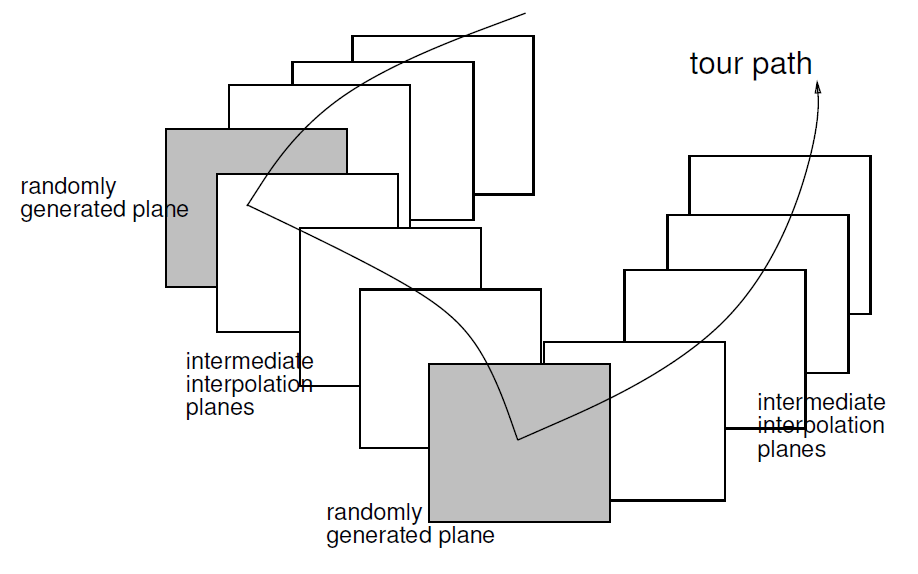
\includegraphics[width=0.8\linewidth,]{figures/buja05fig} 

}

\caption{Simlified illustration of a grand tour target and interim frames  (Buja et al. 2005)}\label{fig:grandFrames}
\end{figure}

The \emph{guided} tour (Cook, Buja, and Cabrera 1993) makes use of projection pursuit (Kruskal 1969, 1972) to identify a path. Here a selected index function is selected. Starting from the initial basis several nearby bases are checked to see if they perform better on the index function. If so, this new basis is moved and nearby bases are checked again in an iterative process. If the closest bases do not perform better, bases slightly further away are checked as in simulated annealing (Kirkpatrick, Gelatt, and Vecchi 1983). If no better basis is identified within the selected stopping criterium, the algorithm stops.

The discrete methods above identity bases that highlight some feature. The above tours can help understand the structure leading to and from certain projections. To explore higher dimensional spaces visually, we need \emph{human-in-the-loop} (Karwowski 2006) tools. We need to be able to choose and direct the change to a basis. (Cook and Buja 1997) introduces the idea of the \emph{manual} tour. In a manual tour, an individual variable is selected and its contribution to the projection basis is then controlled. The manual tour can play a predefined manual path or be used interactively, where the user defines each subsequent step while viewing the current projection. The later, human-in-loop method we define as \emph{User-Controlled Steering} (UCS) specifically as the interactive application of the manual tour.

\hypertarget{research-objectives}{%
\subsection{Research objectives}\label{research-objectives}}

Data and models are typically high-dimensional, with many variables and parameters. Developing new methods to visualize high dimensions has been a pursuit of statisticians, computer scientists and visualization researchers for decades. As technology evolves examining, extending, and assessing current techniques, in new environments, for new data challenges, is an important endeavor. The primary Research Objectives (RO) can then be summarized as the following.

\textbf{\#TODO: reword ``ideal form'', drop to contribution? discuss with Di tomrorrow.}
1. \textbf{What is the ideal form of an interoperable application of manual tour?}\\
An algorithm for the manual tour is discussed in Cook and Buja (1997). The algorithm should be better supported, especially proof for the rotation matrix identified. An application of this ideally embodies two properties: interoperable with other tour applications and allow for `next step' interaction for UCS. Manual tours, and specifically the fine control of UCS, should allow analysts to better explore the sensitivity of structure from single variable contributions on the projection. This also acts as the foundation to be used in the remaining objectives.

\begin{enumerate}
\def\labelenumi{\arabic{enumi}.}
\setcounter{enumi}{1}
\item
  \textbf{Do 2D interactive manual tours provide benefits over alternatives?}\\
  User-control manipulation around identified projections of interest theoretically allows for a better understanding of the variables contributing to the structure. However, the level of abstraction and the sheer number of basis permutations is formidable. The idea that UCS will provide digestible improvements to the understanding of structure should be validated.
\item
  \textbf{How can the manual tour be extended to 3D?}\\
  Gracia et al. (2016) compares analyst tasks between 2- and 3-D scatterplots. They find modest accuracy and error improvements for distance perception and outlier identification in favor of 3D at the cost of a relatively small increase in task time. Nelson, Cook, and Cruz-Neira (1998) similarly compare a 2D scatterplot projection and the 3D scatterplot manipulation space (of the same projection). They find a slight advantage in the sphere test and a large advantage in the cluster test in favor of the 3D manipulation space. The manual tour should be extended to accommodate a 3D projection as analogous improvements may be obtainable.
\item
  \textbf{Do 3D manual tours provide benefits over alternatives?}\\
  \textbf{\#TODO: add here, can we use the same data? same app? same idea as RO2?}
\end{enumerate}

\hypertarget{methodology}{%
\subsection{Methodology}\label{methodology}}

This research is interdisciplinary; touring was developed by statisticians to explore physics data. Modern advances in hardware from information technology allow for 3D rending in higher quality and immersion than previously possible.

The research corresponding with RO \#1 entails \emph{algorithm design} following and further clarifying the work done in Cook and Buja (1997). In the application of the manual tour, we clarified the creation of the rotation matrix. The key to the matrix is to specify the 2 axes of rotation for the manipulation space and apply Rodrigues' rotation formula (Rodrigues 1840). In the application, attention was given to both pre-compiled tour and human-in-the-loop UCS. We provide an open-source version of the manual tour in the R package, \texttt{spinifex}, which has since been published on CRAN. This forms the foundation for future work in the remaining objectives.

For RO \#2 is a controlled \emph{experimental study} to explore the efficacy of interactive UCS compared with the benchmarks factors of PCA and the grand tour. This is designed as a within-participant study where each participant performs all factors. the study is balanced by assigning participants into one of 3 groups where the factor order is controlled by a Latin square while simulation order remains the same. The details are discussed in finer detail in section (\#sec:expStudy), below.

The research for RO \#3 involves \emph{algorithm design} extending the current 2D manual tour into a 3D project. For a 2D projection, the axes basis is rotated through a 3D `manipulation space'. In a 3D projection, such a space requires 4 dimensions. Theoretically, after the addition of a new angle of rotation, the rotation matrix must be extended to accommodate a new dimension and angle parameter. This also means that analysts have another parameter to define, further increasing their already sizable input-volume.

\hypertarget{progress-since-confirmation}{%
\section{Progress since confirmation}\label{progress-since-confirmation}}

During the candidature confirmation review (27 March 2019) we discussed exploratory data analysis, visualization of high dimensional spaces, covered the literature for tours and 3D rendering for information perception. We concluded with a process for a manual tour that allows for user-controlled steering. The appending the document was a mostly complete R package and respective paper providing an open-source application as well as clarifying the rotation matrix that was outlined in Cook and Buja (1997).

\hypertarget{publication}{%
\subsection{Publication}\label{publication}}

The paper has since been accepted in the R Journal and it currently undergoing editorial review. This will be published in the first issue of 2020 and available at \href{https://journal.r-project.org/}{journal.r-project.org}.

\hypertarget{software}{%
\subsection{Software}\label{software}}

The R package, \texttt{spinifex\ (v0.1.0)} (Spyrison and Cook 2019), has been approved and hosted for public use on the Comprehensive R Archival Network, CRAN (cran.r-project.org/web/packages/spinifex/)(\url{https://cran.r-project.org/web/packages/spinifex/index.html}).

New functionality has been added to the development branch, specifically around the interactive use. A user application is developed with \texttt{shiny}(Chang et al. 2018). It allows users to explore their data without the need for coding familiarity. It features interactive or precompiled manual touring. It also contains a gallery for flagging bases which can then further be reviewed or saved as .gif and .png files.

\hypertarget{sec:expStudy}{%
\subsection{Experimental study}\label{sec:expStudy}}

The prominent appeal of the manual tour is that it allows users to control the contributions of individual variables. In theory, this should enable the finer exploration of features of interest. The hypothesis we will study is \emph{Does the finer control afforded by the manual tour improve the ability of the analyst to understand the importance of variables contributing to the structure?}

We list out an abbreviated summary of the experimental design in the subsections below. A more detailed draft of the working paper is included as an appendix.

\hypertarget{sec:groups}{%
\subsubsection{Groups}\label{sec:groups}}

Each participant will be randomly split into one of three even groups. The group controls the order of the factors that the participant was evaluated in for a latin square of the 3 factors. For instance, the order of the first group was PCA, grand, manual. Group level only impacts the order the factors are displayed while task, block, and simulation order will remain the same.

\begin{figure}[h]

{\centering 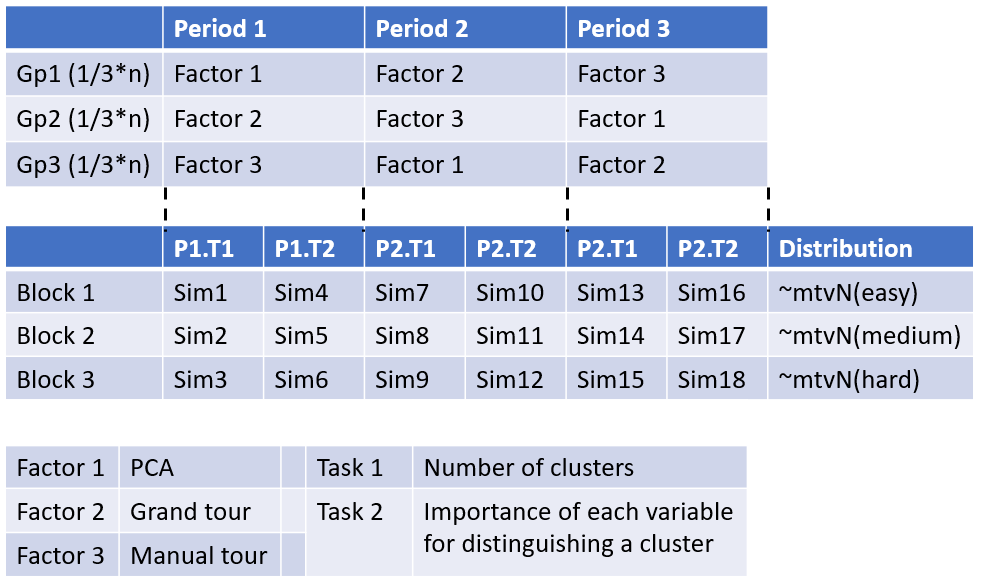
\includegraphics[width=0.8\linewidth,]{./figures/experimental_design} 

}

\caption{Experimental design setup. Participants are assigned to one of 3 even groups controlling the factor order. Within each factor, users perform 3 difficulty blocks of task 1 and then of task 2 before proceeding to the next factor. Simulations are used in a fixed order (while factor order changes). Simulations for the first block difficulty are unique samples drawn from the same distribution. Similarly, the second and third block difficulties are drawn from increasing complex distributions.}\label{fig:design}
\end{figure}

\begin{figure}[h]

{\centering 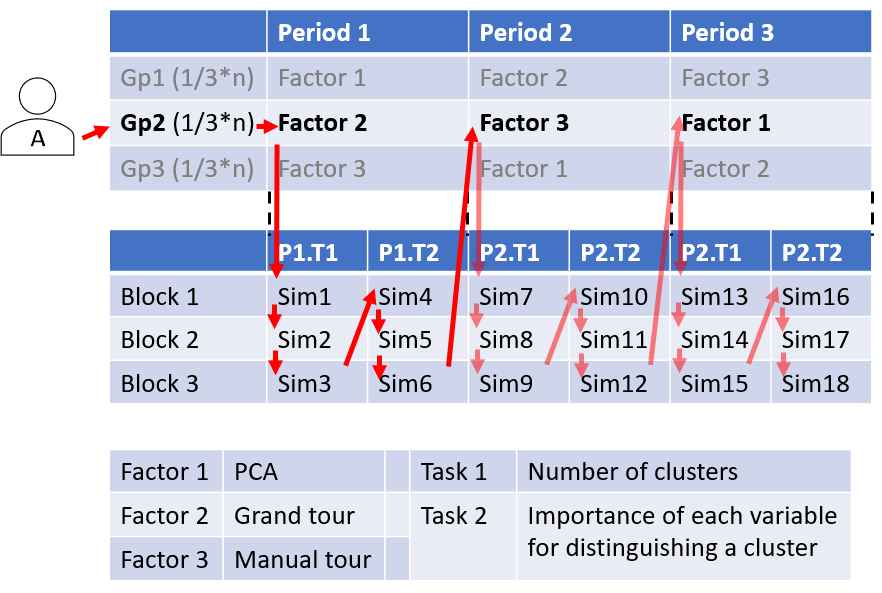
\includegraphics[width=0.8\linewidth,]{./figures/experimental_design_personA} 

}

\caption{Example case. Person 'A' is assigned to group 2, where they will use factor 2 (grand tour) for the first period. They perform 3 block difficulties of task 1 on simulations of increasing difficulty. Then 3 block difficulties of task 2 on unique simulations sampled from the same distributions of increasing difficulty. After this, they proceed to period 2, where they are use factor 3 (manual tour) to perform 3 block difficulties of each task. Lastly, in the third period, they use factor 1 (PCA) to perform the tasks.}\label{fig:designExample}
\end{figure}

\hypertarget{sec:factors}{%
\subsubsection{Factors}\label{sec:factors}}

We will explore performance across three factors. The first factor is Principal Component Analysis (PCA). The second factor is an animated walk of interpolation frames between target bases, called a \emph{grand} tour. The third factor allows for the manual control of the individual variable's contribution to the projection, performing a \emph{manual} tour.

All factors are shown as a scatterplot. The basis axes projection was also illustrated to the left of the plot. They are shown in a unit circle and show the magnitude and direction each variable contributes to the projection.

The user interface was kept the same whenever possible, but the control inputs do change slightly to accommodate the differences between factors. The inputs for PCA select a pair of principal components to display on the x- and y-axes. The manual tour had the same axes selection, with the addition of a drop-down bar and slider control selecting the manipulation variable and magnitude. The grand tour comes precompiled as an animation of a 15 second showing 90 frames at 6 frames per second. The user can control the location or play/pause the animation at will.

\hypertarget{sec:tasks}{%
\subsubsection{Tasks}\label{sec:tasks}}

Within each factor, participants will perform 2 tasks. The first task asks participants to identify the number of clusters present in unsupervised data. This task served as a standard for assessing the general aptitude for this sort of high dimensional analysis as it was simpler. In application, linear discriminant analysis (Fisher 1936) or penalized discriminant analysis (Hastie, Buja, and Tibshirani 1995) are better suited for classifying such unsupervised data.

The second task is focused on the hypothesis of the study, it asks participants to identify any/all variables that were very important and somewhat important for distinguishing a given cluster from the others. For instance, which variables are very- and somewhat- important for distinguishing clusters `A' and `B'.

\hypertarget{sec:blocks}{%
\subsubsection{Block difficulty}\label{sec:blocks}}

Participants will be randomly assigned to 1 of 3 even groups. Each group has a different factor order containing all factors. Both tasks will be performed in the same order. Each task will have 3 repetitions performed on new simulations that were drawn from 3 parameterizations in increasing difficulty. Each participant will go through the simulations in the same order, while their factor order will vary. Fixing block difficulty order while varying factors should mitigate potential learning bias.

\hypertarget{proposed-thesis-structure}{%
\section{Proposed thesis structure}\label{proposed-thesis-structure}}

\hypertarget{thesis-structure}{%
\subsection{Thesis structure}\label{thesis-structure}}

\begin{itemize}
\tightlist
\item
  Introduction -- 60\%
\item
  Literature review -- 80\%
\item
  Manual tour and user-controlled steering -- 90\%
\item
  Experimental study -- 60\%
\item
  The extension of the manual tour to 3D -- 5\%
\item
  Conclusion and future plans -- 0\%
\end{itemize}

\textbf{Proposed research timeline}

\begin{figure}[h]

{\centering 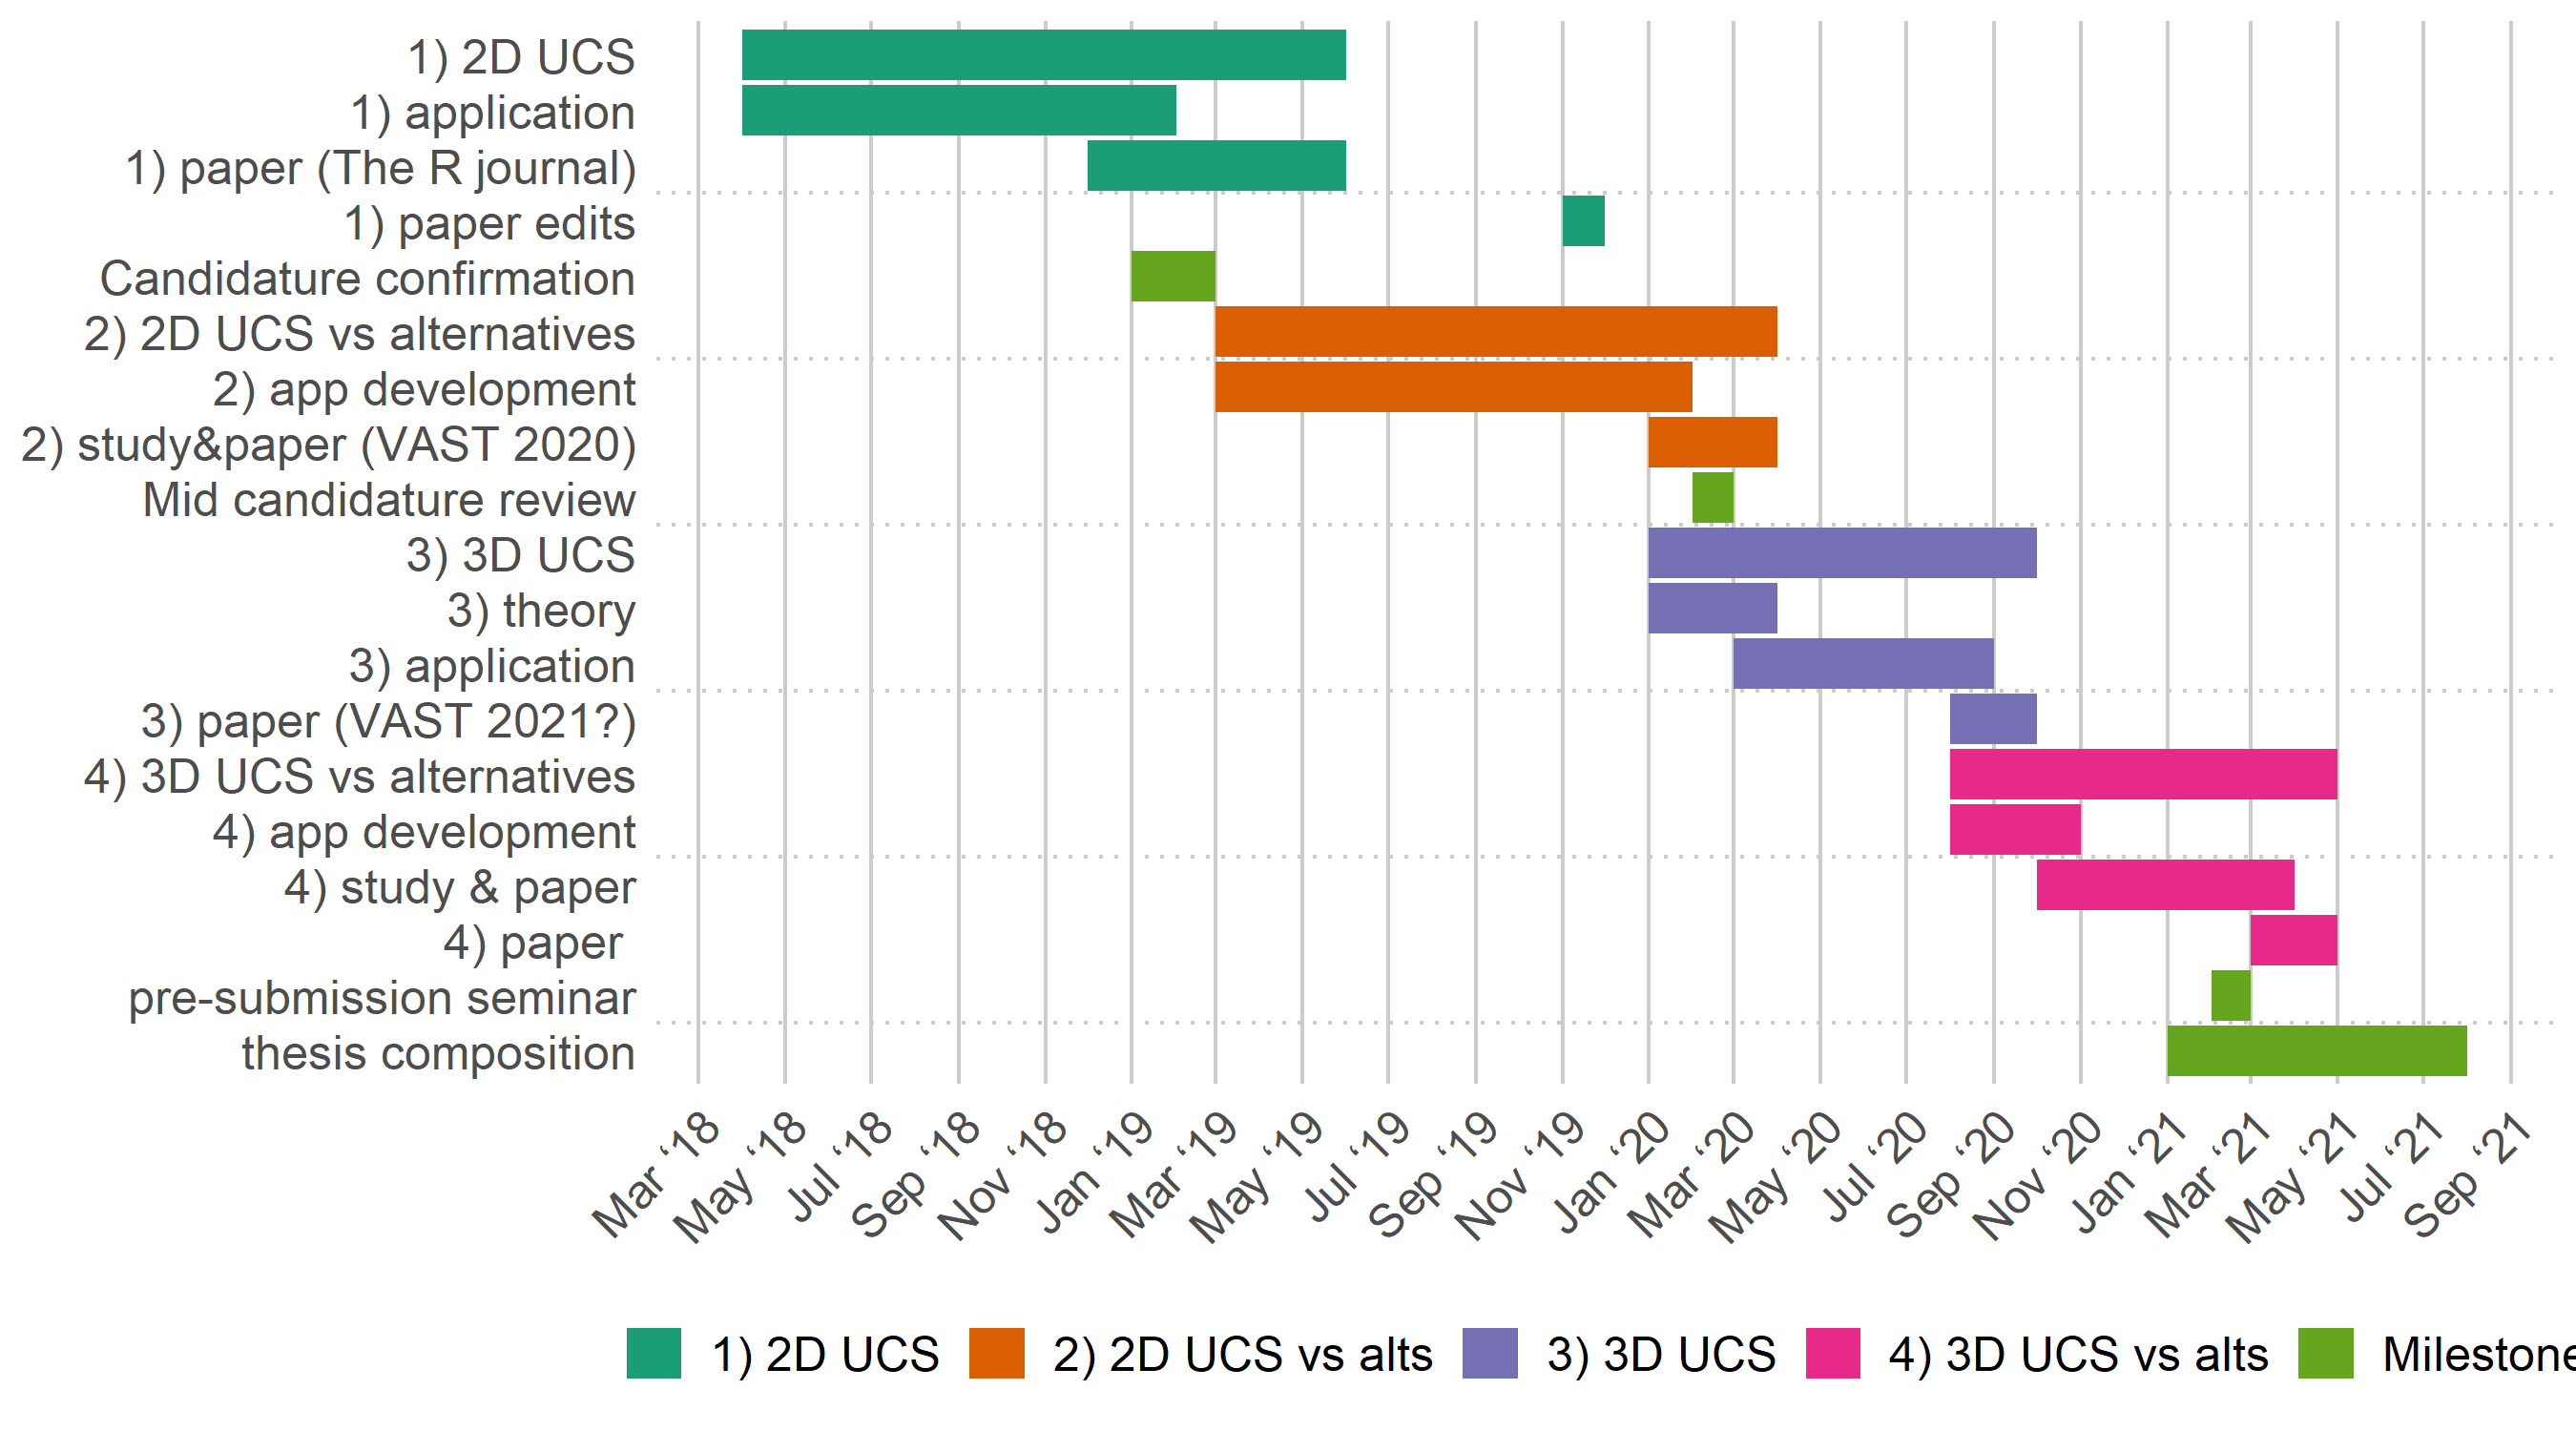
\includegraphics[width=1\linewidth,]{figures/phd_timeline} 

}

\caption{Proposed research timeline.}\label{fig:timeline}
\end{figure}

\hypertarget{program-requirements}{%
\subsection{Program requirements}\label{program-requirements}}

\begin{itemize}
\tightlist
\item
  WES Academic record

  \begin{itemize}
  \tightlist
  \item
    FIT5144: 2019 S1+2, \textbf{In progress}, extended to the pre-submission seminar with the unit coordinator for the usual 2 opportunities to complete.

    \begin{itemize}
    \tightlist
    \item
      Hours: 147\textgreater120 hours \textbf{Tracked}, missing the following requirments (12 hr total)
    \item
      \emph{Needed:} CYR 2 (A \& B) -- 2x 3hr
    \item
      \emph{Needed:} Faculty of IT Workshop 1 and 3 on Ethical Research and Publishing -- 2x 3hr
    \end{itemize}
  \item
    FIT5113: 2018 S2, \textbf{Exemption}
  \item
    FIT6021: 2018 S2, \textbf{Completed} with distinction
  \end{itemize}
\item
  myDevelopment - IT: Monash Doctoral Program - Compulsory Module

  \begin{itemize}
  \tightlist
  \item
    Monash graduate research student induction: \textbf{Completed}
  \item
    Research Integrity - Choose the Option most relevant: \textbf{Completed}
  \item
    Faculty Induction: \textbf{Completed}
  \end{itemize}
\end{itemize}

\hypertarget{potential-issues-for-panel-to-consider}{%
\section{Potential issues for panel to consider}\label{potential-issues-for-panel-to-consider}}

\hypertarget{funding-for-human-subjects}{%
\subsection{Funding for human subjects}\label{funding-for-human-subjects}}

\begin{itemize}
\tightlist
\item
  Beverage voucher: \$5 x 24 people (est) = \$120
\end{itemize}

\hypertarget{support-for-conference-travel}{%
\subsection{Support for conference travel}\label{support-for-conference-travel}}

\textbf{Conferences:}\\
~\\
CHI 2021: May 8-13, 2021 Yokohama, Japan\\
submission: Thursday Sep.~10, 2020\\
\url{https://chi2021.acm.org/}~\\
~\\
IEEE VAST - VAST 2020: 25-30 October 2020 Salt Lake City, Utah, USA\\
submission: Saturday, March 21, 2020\\
\url{http://ieeevis.org/year/2020/info/call-participation/vast-paper-types}

\hypertarget{sec:acknowledgements}{%
\section{Acknowledgements}\label{sec:acknowledgements}}

This report was created in \texttt{R} (R Core Team 2019), using \texttt{bookdown} (Xie 2016) and \texttt{rmarkdown} (Xie, Allaire, and Grolemund 2018).

For version control, transparency, and reproducibility, the source files are made available found at \href{https://github.com/nspyrison/mid_canidature}{github.com/nspyrison/mid\_canidature}.

\hypertarget{references}{%
\section*{References}\label{references}}
\addcontentsline{toc}{section}{References}

\hypertarget{refs}{}
\leavevmode\hypertarget{ref-anscombe_graphs_1973}{}%
Anscombe, F. J. 1973. ``Graphs in Statistical Analysis.'' \emph{The American Statistician} 27 (1): 17--21. \url{https://doi.org/10.2307/2682899}.

\leavevmode\hypertarget{ref-asimov_grand_1985}{}%
Asimov, Daniel. 1985. ``The Grand Tour: A Tool for Viewing Multidimensional Data.'' \emph{SIAM Journal on Scientific and Statistical Computing} 6 (1): 128--43. \url{https://doi.org/https://doi.org/10.1137/0906011}.

\leavevmode\hypertarget{ref-buja_grand_1986}{}%
Buja, Andreas, and Daniel Asimov. 1986. ``Grand Tour Methods: An Outline.'' In \emph{Proceedings of the Seventeenth Symposium on the Interface of Computer Sciences and Statistics on Computer Science and Statistics}, 63--67. New York, NY, USA: Elsevier North-Holland, Inc. \url{http://dl.acm.org/citation.cfm?id=26036.26046}.

\leavevmode\hypertarget{ref-cattell_scree_1966}{}%
Cattell, Raymond B. 1966. ``The Scree Test for the Number of Factors.'' \emph{Multivariate Behavioral Research} 1 (2): 245--76.

\leavevmode\hypertarget{ref-chambers_graphical_1983}{}%
Chambers, J. M., W. S. Cleveland, B. Kleiner, and P. A. Tukey. 1983. ``Graphical Methods for Data Analysis.''

\leavevmode\hypertarget{ref-chang_shiny:_2018}{}%
Chang, Winston, Joe Cheng, J. J. Allaire, Yihui Xie, and Jonathan McPherson. 2018. \emph{Shiny: Web Application Framework for R}. \url{https://CRAN.R-project.org/package=shiny}.

\leavevmode\hypertarget{ref-cook_manual_1997}{}%
Cook, Dianne, and Andreas Buja. 1997. ``Manual Controls for High-Dimensional Data Projections.'' \emph{Journal of Computational and Graphical Statistics} 6 (4): 464--80. \url{https://doi.org/10.2307/1390747}.

\leavevmode\hypertarget{ref-cook_projection_1993}{}%
Cook, Dianne, Andreas Buja, and Javier Cabrera. 1993. ``Projection Pursuit Indexes Based on Orthonormal Function Expansions.'' \emph{Journal of Computational and Graphical Statistics} 2 (3): 225--50. \url{https://doi.org/10.1080/10618600.1993.10474610}.

\leavevmode\hypertarget{ref-fisher_use_1936}{}%
Fisher, Ronald A. 1936. ``The Use of Multiple Measurements in Taxonomic Problems.'' \emph{Annals of Eugenics} 7 (2): 179--88. \url{https://doi.org/10.1111/j.1469-1809.1936.tb02137.x}.

\leavevmode\hypertarget{ref-gracia_new_2016}{}%
Gracia, Antonio, Santiago González, Víctor Robles, Ernestina Menasalvas, and Tatiana von Landesberger. 2016. ``New Insights into the Suitability of the Third Dimension for Visualizing Multivariate/Multidimensional Data: A Study Based on Loss of Quality Quantification.'' \emph{Information Visualization} 15 (1): 3--30. \url{https://doi.org/10.1177/1473871614556393}.

\leavevmode\hypertarget{ref-hastie_penalized_1995}{}%
Hastie, Trevor, Andreas Buja, and Robert Tibshirani. 1995. ``Penalized Discriminant Analysis.'' \emph{The Annals of Statistics}, 73--102.

\leavevmode\hypertarget{ref-karwowski_international_2006}{}%
Karwowski, Waldemar. 2006. \emph{International Encyclopedia of Ergonomics and Human Factors, -3 Volume Set}. CRC Press.

\leavevmode\hypertarget{ref-kirkpatrick_optimization_1983}{}%
Kirkpatrick, Scott, C. Daniel Gelatt, and Mario P. Vecchi. 1983. ``Optimization by Simulated Annealing.'' \emph{Science} 220 (4598): 671--80. \url{https://doi.org/10.1126/science.220.4598.671}.

\leavevmode\hypertarget{ref-kohonen_self-organizing_1990}{}%
Kohonen, Teuvo. 1990. ``The Self-Organizing Map.'' \emph{Proceedings of the IEEE} 78 (9): 1464--80.

\leavevmode\hypertarget{ref-kruskal_toward_1969}{}%
Kruskal, Joseph B. 1969. ``Toward a Practical Method Which Helps Uncover the Structure of a Set of Multivariate Observations by Finding the Linear Transformation Which Optimizes a New `Index of Condensation'.'' In \emph{Statistical Computation}, edited by Roy C. Milton and John A. Nelder, 427--40. Academic Press. \url{https://doi.org/10.1016/B978-0-12-498150-8.50024-0}.

\leavevmode\hypertarget{ref-kruskal_linear_1972}{}%
---------. 1972. ``Linear Transformation of Multivariate Data to Reveal Clustering.'' \emph{Multidimensional Scaling: Theory and Applications in the Behavioral Sciences} 1: 181--91.

\leavevmode\hypertarget{ref-maaten_visualizing_2008}{}%
Maaten, Laurens van der, and Geoffrey Hinton. 2008. ``Visualizing Data Using T-SNE.'' \emph{Journal of Machine Learning Research} 9 (Nov): 2579--2605.

\leavevmode\hypertarget{ref-matejka_same_2017}{}%
Matejka, Justin, and George Fitzmaurice. 2017. ``Same Stats, Different Graphs: Generating Datasets with Varied Appearance and Identical Statistics Through Simulated Annealing.'' In \emph{Proceedings of the 2017 CHI Conference on Human Factors in Computing Systems - CHI '17}, 1290--4. Denver, Colorado, USA: ACM Press. \url{https://doi.org/10.1145/3025453.3025912}.

\leavevmode\hypertarget{ref-nelson_xgobi_1998}{}%
Nelson, Laura, Dianne Cook, and Carolina Cruz-Neira. 1998. ``XGobi Vs the C2: Results of an Experiment Comparing Data Visualization in a 3-d Immer- Sive Virtual Reality Environment with a 2-d Workstation Display.'' \emph{Computational Statistics} 14 (1): 39--52.

\leavevmode\hypertarget{ref-pearson_liii._1901}{}%
Pearson, Karl. 1901. ``LIII. On Lines and Planes of Closest Fit to Systems of Points in Space.'' \emph{The London, Edinburgh, and Dublin Philosophical Magazine and Journal of Science} 2 (11): 559--72.

\leavevmode\hypertarget{ref-r_core_team_r:_2019}{}%
R Core Team. 2019. \emph{R: A Language and Environment for Statistical Computing}. Vienna, Austria: R Foundation for Statistical Computing. \url{https://www.R-project.org/}.

\leavevmode\hypertarget{ref-rodrigues_lois_1840}{}%
Rodrigues, Olinde. 1840. \emph{Des Lois Géométriques Qui Régissent Les Déplacements d'un Système Solide Dans L'espace: Et de La Variation Des Cordonnées Provenant de Ces Déplacements Considérés Indépendamment Des Causes Qui Peuvent Les Produire}.

\leavevmode\hypertarget{ref-spyrison_spinifex_2019}{}%
Spyrison, Nicholas S., and Dianne Cook. 2019. \emph{Spinifex: Manual Tours, Manual Control of Dynamic Projections of Numeric Multivariate Data} (version 0.1.0.9000). \url{https://github.com/nspyrison/spinifex/}.

\leavevmode\hypertarget{ref-tukey_exploratory_1977}{}%
Tukey, John W. 1977. \emph{Exploratory Data Analysis}. Vol. 32. Pearson.

\leavevmode\hypertarget{ref-wickham_tourr:_2011}{}%
Wickham, Hadley, Dianne Cook, Heike Hofmann, and Andreas Buja. 2011. ``Tourr: An R Package for Exploring Multivariate Data with Projections.'' \emph{Journal of Statistical Software} 40 (2). \url{https://doi.org/10.18637/jss.v040.i02}.

\leavevmode\hypertarget{ref-xie_bookdown:_2016}{}%
Xie, Yihui. 2016. \emph{Bookdown: Authoring Books and Technical Documents with R Markdown}. Boca Raton, Florida: Chapman; Hall/CRC. \url{https://github.com/rstudio/bookdown}.

\leavevmode\hypertarget{ref-xie_r_2018}{}%
Xie, Yihui, J. J. Allaire, and Garrett Grolemund. 2018. \emph{R Markdown: The Definitive Guide}. Boca Raton, Florida: Chapman; Hall/CRC. \url{https://bookdown.org/yihui/rmarkdown}.

\end{document}
